\chapter{The Chronograph Platform}
\label{chp:chrono}

The foregoing chapters of this thesis described how retroactive capabilities 
with an ES+CQRS style of architecture can be utilized. In this chapter, we 
examine if and how the results from the previous chapters can be transferred 
to an event-sourced system with a different architectural style. The 
Chronograph research platform is the subject of this examination.

\section{Background}
Chronograph \cite{Erb2015} is an event-sourced, distributed platform with the 
underlying structure of a graph.
The platform thus has potential retroactive capabilities, which have not been 
considered so far. Events are only ever appended, but no retroaction is applied. 
The programming model is vertex-centric, each vertex in the graph possesses an 
individually specified behavior -- the \emph{behavior function}. Vertices 
communicate via asynchronous message passing with their neighbors, can spawn 
new vertices, and create or remove edges. 
%
A message addressed to a vertex triggers the processing of this message within 
the vertex. Such a computation can result in changes to the vertex state, 
modifications to the vertex edges, the spawning of new vertices, or outgoing 
messages. State changes are persisted as events into an event log which 
belongs to the vertex. Thus, event sourcing is the mean to persist vertex 
state. The behavior function is part of the vertex state and is also persisted 
with the event. It can be exchanged dynamically by the vertex. 
Formally, a vertex at a time $t$ can be described as reacting to an incoming 
message $m$ by invoking its current behavior function $f_t$. The function 
returns the updated state and a (possibly different) behavior function:

\begin{quote}
\centering
$ (S_{t+1}, f_{t+1}) = f_t (m, S_t)$
\end{quote}

\noindent{}A pseudo code implementation of this formal description can be 
written like this:

\begin{lstlisting}[
	style=styled, 
]
vertices["foo"].behaviorFn = function(state, msg) {
	// local computations
	state.foo = state.bar + 1;

	return [state, vertices["foo"].behaviorFn];
}
\end{lstlisting}

The behavior function of this vertex ``\cmd{foo}'' is invoked once an incoming
message is available. The prior vertex state is supplied to the behavior function 
as an argument. The function then processes the message and returns the updated 
state object, as well as the subsequent behavior function.

In Chronograph, a runtime engine is responsible for providing underlying 
services (message passing, persistence, calculating events, etc.). Multiple 
instances (i.e. workers) can be connected, in order to distribute a graph over 
multiple machines or processes (Figure \ref{fig:chronograph}).

\begin{figure}
	\centering
	\includegraphics[page=3,width=0.9\textwidth]{../illustrations/chronograph.pdf}
	\caption{
		In Chronograph, vertices can be spread over multiple workers, which do not 
		necessarily have to run on the same physical machine.
	}
	\label{fig:chronograph}
\end{figure}

\section{Differences to Prior Architectures}
The event-sourced architectures, which we described in Chapters \ref{chp:concept}
and \ref{chp:programming} have some differences to the Chronograph architecture.
Before we examine the application of retroaction in Chronograph further, we 
examine these differences first.


\subsection{Local vs. Global View}
In Chronograph each vertex possesses a local view. It can communicate with 
neighbors, modify its edges, and spawn new vertices, but its computation takes 
only the local vertex state and arriving messages into consideration. 
This is basically the scenario we viewed in Chapter \ref{chp:concept} and
\ref{chp:programming}, where we considered a system which receives commands 
from an outside world.
The IoT scenario, which we used to illustrate our conceptual considerations
in Chapter \ref{chp:concept}, is a use case which suits well for Chronograph.
Independent IoT devices can be modelled as vertices in a graph. The devices
are connected via edges and communicate via asynchronous message passing.
Devices are independent from each other; each one possesses an individual 
behavior function and its own timeline. Though, each device is loosely coupled 
to nearby devices and there might be causal dependencies among devices.
In this IoT scenario, the local view refers to the view of one device on itself.

But in Chronograph a global view exists as well. Vertices are interconnected 
via edges and form a graph topology. This topology restrains the communication 
possibilities, since only neighboring vertices can communicate with each other. 
If retroaction is applied to the graph, new challenges emerge:
There is no global timeline, logic, or event log -- each vertex possesses its 
own. The global view only emerges when the graph is examined in its entirety.
For this, multiple event logs need to be taken into account and the creation of 
a consistent graph snapshot is necessary.
The issue of creating snapshots in distributed event-sourced has been addressed 
by Habiger \cite{Habiger2015} in 2015.
In our IoT scenario, a global view could be calculated by a controller device 
which keeps track of all devices.

\subsection{CQRS in Chronograph}
Chronograph possesses a segregation of commands and queries as well. But the
implementation differs from our prior architectures.
Commands are sent by vertices to vertices, but queries are issued from an 
underlying platform. Queries take place outside of the graph, on a different 
layer than commands.
Behavior functions are written by a programmer to specify the behavior of 
vertices. Within a behavior function, incoming messages are processed, state 
may be mutated, and new messages sent.
Queries on the other hand are issued from the runtime engine (e.g. by an 
administrator) and refer to the state of the entire graph. There is usually 
a snapshot mechanism, which yields a consistent state of the graph, involved.

Messages in Chronograph can be considered what we previously described as 
commands. Here, messages which are passed between vertices trigger a computation 
within a vertex, and thus possibly an internal state change. 
To summarize: Queries and commands are also viewed as separate operations, but a 
query happens on the snapshot of a graph and is decoupled from the application
itself. Commands, on the other hand, are sent as messages between vertices.

\section{Retroaction in Chronograph}
This section examines how retroaction can be achieved in the platform. For this, 
we apply the ideas introduced in Chapters \ref{chp:concept} and 
\ref{chp:programming}, in order to utilize temporal aspects of the platform. 
There are a number of use case which motivate retroaction in Chronograph. 

\paragraph{Retroactive Insights}
Past states of the graph can be explored. This can be used for analysis purposes
and the results can be utilized to e.g. change the future behavior of the system. 

\paragraph{Compare Behavior Functions}
It can be examined how different behavior functions would have affected the 
system. This can be achieved  by replaying the messages from the graph's 
history, with different behavior functions for vertices. 

\paragraph{Messages}
Messages can be retroactively inserted or deleted, to examine how they would 
have affected the graph's state.

\paragraph{Topology Changes}
Topology changes can be applied retroactively to examine the impact of a different 
graph topology.

\ \\
An example of a retroactive application in the IoT scenario, is to retroactively 
explore how different behavior functions in individual devices would have affected 
the system state.

\subsection{Behavior Function vs. Runtime Engine}
In Chronograph, access to retroaction can be exposed either (1) in the behavior 
function or (2) in the underlying runtime engine. In case of (1), this leads to 
a similar programming model as in Chapter \ref{chp:programming}.


\subsection{Local vs. Global}
Causalities in Chronograph occur, when (1) local state is read or mutated and 
(2) when messages are sent or received.
When messages are exchanged with neighboring vertices, they trigger computations, 
which in turn might modify state and dispatch new messages. In contrast to the 
systems in Chapters \ref{chp:concept} and \ref{chp:programming}, this implies 
that causalities occur to a larger degree outside the local view of a vertex. 
Thus, to fully utilize the expressiveness of retroaction, the entire graph needs 
to be taken into account. In replays, hidden causalities can otherwise occur in 
neighbors of a vertex: Since the vertices outside of a vertex would not be newly
computed, there is no coupling with them -- messages sent to them would not be 
processed and thus not influence the replay. 
If retroactive changes are applied in only one vertex this can weaken the 
informative value. Side effects can be a reason for further hidden causalities.

It is actually possible to apply a lot of the ideas from the previous chapters 
to Chronograph -- if we just examine the local view in a vertex we can apply 
our insights from Chapters \ref{chp:concept} and \ref{chp:programming}. 
Though, hidden causalities in the graph outside of a vertex can have a limiting 
effect. Through the interaction of the graph with the outside world (through 
side effects), additional hidden causalities might exist. Thus, we cannot limit 
retroactive capabilities to a local vertex, the nature of the graph rather has 
to be taken into account when utilizing retroaction in Chronograph.

Besides the primitives of retroaction which we described in the programming 
model from Chapter \ref{chp:programming}, Chronograph has an additional 
retroactive primitive which allows to retroactively edit the topology.
Transferred to the IoT scenario, this allows to explore how a different
topology would have influenced the system.
For example, individual devices might have chosen for different actions if
neighboring devices would have been available.

\section{Proposals to Implement Retroaction}
Some of the concepts, which we applied for implementing retroaction in 
event-sourced systems, can be applied to Chronograph as well.
In Chapter \ref{chp:concept}, we argued that causality violations occur when 
a timeline modifies its own past. Furthermore, directly editing the past 
contradicts the append-only nature of event-sourced systems and breaks with 
its benefits for e.g. scalability or traceability.
Thus, we proposed to distinguish between a \emph{main timeline} and its 
\emph{branches}. We restricted direct editing to branches and retained the 
append-only behavior for the main timeline.
The same reasons hold true for Chronograph and we propose to apply the 
differentiation of a main timeline with branches in Chronograph as well. 

\pagebreak
\subsection{Side Effects}
As described in Section \ref{sec:side-effects}, side effects pose a challenge 
to retroaction. They can have a negative effect in replays, since they can be 
a source for hidden causalities. This can be the reason that the system behaves 
unforeseeable differently in a replay. 
Side effects are also tricky in terms of control in replays. It has to be 
possible to (1) suppress their invocation, (2) reuse the result from the 
original invocation, and (3) reinvoke them and use the new result for the 
further processing. In Section \ref{sec:replaying-se}, we proposed the concept 
of partial replays to impose control over side effects. 
To briefly recapitulate on the core insights: We excavated side effects from 
within application commands, instead they were placed in individual commands 
with few application logic. 
This concept allows for handling side effects with system primitives, they were 
invoked as commands and their results recorded as events.
We also highlighted that through this splitting of large commands into a series 
of commands and side effect afflicted commands, three constraints follow: 

\begin{enumerate}
\item Few logic is executed when the series is issued, only the success and
failure of commands is checked. Otherwise, this logic layer would not be 
persisted to the timeline and would not be taken into account in a command 
replay.

\item Each command in this series needs to be persisted to the timeline, 
independent of its success or failure. This way a later replay can re-execute 
this series with a modified processing logic.

\item The commands in this series need to be invoked in a serializable order.
A non-serialized replay may break the deterministic cause of events.
\end{enumerate}

This concept can be transferred to Chronograph, by excavating side effect
operations from the behavior function into separate vertices. These operations
can then be dispatched via asynchronous message passing.
Vertices conduct the side effect afflicted operations and return the result
via asynchronous messages. This way the invocation message and the resulting 
data are persisted in the timeline. Thus, in a replay it is possible to control 
if the result from the original invocation should be reused (i.e. the persisted 
message which returned), or if the side effect operation should be executed 
again (i.e. the message sent to the vertex again).

But it is not sufficient to solely place side effect operations within separate 
vertices -- these vertices also need a special role. They cannot be treated like 
normal Chronograph vertices, since a vertex which performs I/O operations cannot 
be restored to an arbitrary state.
A vertex could e.g. perform the function of processing data from the TCP 
connection of a live stream; restoring an arbitrary state of this TCP connection 
is generally not possible. Thus the usage of \emph{I/O vertices} becomes 
necessary. In terms of communication via asynchronous messages, spawning them, 
and programming them, these I/O vertices act like normal vertices. But they do 
not return or persist state.
The type of a vertex -- normal vertex or I/O vertex -- can be supplied when it 
is initially spawned. The following listing depicts an example how this could be 
implemented. In this example, the behavior function does not utilize I/O vertices,
instead ``normal'' processing logic in the behavior function is blended with side 
effect afflicted operations. A stock price is fetched from a web service and 
depending on the result, the state object is modified and a mail message may be 
sent.

\pagebreak

\begin{lstlisting}[style=styled]
vertices["foo"].behaviorFn = function(state, msg) {
	var stockPrice = http.get("https://.../price");
	if (stockPrice < 500) {
		state.buyingRecommendation = true;
		mail.send("alice@foo.com", "Buying recommendation!");
	}

	return [state, vertices["foo"].behaviorFn];
}
\end{lstlisting}

The problem here is that in a replay neither reusage, nor reinvoking, nor
skipping of the individual side effects can be controlled.
But this behavior function can be re-written to utilize I/O vertices in this
way. In the following listing two special vertices \cmd{stockPriceIO} and
\cmd{mailIO} have been created. The side effect afflicted operations are 
moved to these vertices. The code changes to the original function are marked 
in red. The functionalities can then be triggered by sending messages to these 
vertices. Results are returned to the sender via the native asynchronous 
message passing primitives of Chronograph.

\lstset{moredelim=[is][\color{purple}\itshape]{[*}{*]}}
\begin{lstlisting}[style=styled]
vertices["foo"].behaviorFn = function(state, msg) {
   [*sendMsg("stockPriceIO", "get-price");*]
   if ([*msg.content === "price-fetched"*] && msg.price < 500) {
     state.buyingRecommendation = true;
     [*sendMsg("mailIO", "send-alert-mail");*]
   }
   return [state, vertices["foo"].behaviorFn];
}
 
vertices["stockPriceIO"].behaviorFn = function(msg) {
   if (msg.content === "get-price") {
     var data = http.get("https://.../get-price");
     sendMsg(msg.sender, data);

     return [ vertices["stockPriceIO"].behaviorFn ];
   }
} 
\end{lstlisting}

In a replay, the \cmd{stockPriceIO} function could be exchanged to e.g. 
simulate different I/O by returning simulated stock prices from a fixed list
or fetch them newly from a different server.
In the above example, the function which controls the I/O vertex logic was
described as a behavior function within the system. Since I/O vertices 
are a special type of vertex, the I/O vertex could also be provided by 
the underlying runtime engine. This may allow for more efficient processing
or the coupling with different programming environments (or components).

\subsection{Retroactive Modification}
As a result of a retroactive modification, the state at a point in the vertex 
timeline may have changed. 
In Section \ref{sec:validation} we described possibilities to ensure the 
consistency of the subsequent timeline. Among them were the removal or 
recomputation of causally dependent events. We proposed to annotate the 
system information which was used to compute each event for this. In our 
prototype, this information was defined by the reading and writing operations 
which accessed properties of the system state object. This annotation was 
done manually, by the developer.

This concept can be transferred to Chronograph: We propose for the behavior
function to return the properties of the vertex state object which were
utilized during an invocation of the behavior function.
Though, we propose an improvement of the concept from our prototype: the usage 
of getter and setter methods when accessing properties of the vertex state 
object. These methods are provided by the runtime engine and allow to 
automatically capture which state properties were accessed and modified. 
Through this concept, the developer does not have to annotate this information 
by hand.
Listing \ref{lst:chrono1} illustrates how this concept can be implemented.
A further improvement over the usage of getter and setter methods would be
source code analysis by the underlying runtime engine, to automatically 
annotate this information. Developers would then not have to use setter or 
getter methods, but could rather use normal language syntax.

But this concept is only sufficient to track causal dependencies of a vertex 
in itself. This was sufficient for our prior architectures, in which only a 
single event log existed.
In these prior architectures, commands could not invoke other commands. 
Commands were issued by an application and it was not clear if newly issued 
commands had a causal relationship to previous commands. 
As a consequence, causal dependencies among commands could not be traced, 
although they may have existed. In Chronograph, the underlying model is 
different. Here, vertices can send messages to neighbors. These messages 
trigger a computation in the receiver and result in new events being appended 
to individual event logs. 
Thus, the computation in vertices has a causal relationship to the computation 
of the vertex which sent the message. In case of retroaction, retroactive 
modifications can result in a message no longer being sent. This has 
consequences for the consistency of the timeline, since the neighboring vertex 
then would never have received a message, and thus never executed its 
computation.
This is why direct -- and recursively indirect -- causal dependencies in other 
vertices need to be taken into account when retroactive changes are applied 
(Section~\ref{sec:dependent}). 
In terms of causal dependencies among messages, the concept of vector clocks 
could be applied. Vector clocks can be used to trace causalities among 
messages in a distributed system \cite{Schwarz1994}. 
To ensure a consistent timeline, the computations in vertices which have 
received direct messages and sent subsequent indirect messages, need to be 
recursively removed (or replayed) as well.

\begin{lstlisting}[style=styled,
	caption = {Getter and setter methods can be used to capture causalities 
	among computations. If a retroactive modification is applied, dependent
	computations can be recursively handled. In the case of e.g. a message
	which is retroactively removed, all consequences can be removed from 
	the subsequent timeline as well.},
	label = lst:chrono1
]
vertices["foo"].behaviorFn = function(state, msg) {
	var f = state.get("foo"); /* state.foo */
	state.set("bar", f++);    /* state.bar */

	return [state, vertices["foo"].behaviorFn];
}
\end{lstlisting}

\subsection{Tagging Events and Commands}
In Section \ref{sec:tags}, we described the concept of tagging commands and 
events. We propose to apply this concept in Chronograph as well.
Enabling the tagging of messages \emph{and} events makes sense, since they
both serve a different purpose: 
A message is always issued by the vertex which sends the message; the event 
describes how the vertex who received the message reacts to it. This resulting 
event depends on the behavior function of the receiver. Therefore it makes sense 
to annotate the resulting event with tags \emph{in the behavior function}.
Annotating messages enables us to filter for them, independent of how they
are processed. 
%
For messages, tagging allows to flexibly exclude message categories (or 
individual messages) in replays. This can be used to exclude e.g. messages to 
I/O vertices, in order to prevent side effects from being reinvoked.

Concerning events, tagging allows for an additional use case: creating 
references to certain points in the timeline. These references can be used as 
timeline pointers in retroactive operations (e.g. as branch or insert marks).
Concerning the implementation of tagging, we can utilize the return values
of the behavior function to return tags as well. The following code example 
illustrates how the concept of tagging in the behavior function can work:

\begin{lstlisting}[style=styled]
vertices["foo"].behaviorFn = function(state, msg) {
	var eventTags = [ "branching-point1", "important-data-processed" ];

	var messageTags = [ "some-message-tag" ];
	msg.addTags(messageTags);

	return [state, vertices["foo"].behaviorFn, eventTags];
}
\end{lstlisting}

\subsection{Capturing State Changes in Events}
\label{sec:chronograph-capturing}
In Chronograph, events are implicit changes to a state object. The difference 
before and after the modification is calculated by the underlying platform. 
The persisted event captures these state changes and can be used to rebuild 
state. But the Chronograph specification does not yet define how these deltas 
are encoded.

In the context of retroaction, the form how state changes are encoded is 
important to consider, since this has a large impact on the expressiveness 
and limitations of retroaction. 
In Section \ref{sec:capturing-changes}, we described this impact in detail.
For the reasons described there, the form of JSON Patches suits better for 
Chronograph. Here, the patch contains the operations which were applied -- 
opposed to the mere recording of the result. This allows for retroactive 
changes to \emph{not} be annihilated by subsequent events.
But the issue is not solved completely. JSON Patches record the operation 
which has been applied to an object only in some cases; appending an element
to an array, for example. But in the case of direct value assignments or the 
direct modification of a value at a certain array index, the JSON Patch still 
annihilates retroactive modifications. This is not necessarily an issue, 
but it can have a limiting effect on the insertion of retroactive events and 
commands.

Individual instructions within commands can conflict with prior retroactive 
modifications. For example, in a behavior function a programmer could always 
decrement the value a vertex receives from a certain vertex, relying on some 
knowledge of the context. 
Through retroactive changes, this context may no longer hold and the operation 
thus suddenly have a different semantics.
In Section \ref{sec:rap}, we provided a more detailed examination of this
issue and proposed retroaction-aware programming to provide more semantics to 
instructions. 
This can be done by providing underlying functions to the developer, which 
resolve the ambiguity of instructions (\cmd{getLast()} instead of 
\cmd{object[99]}). This way, conflicts of retroactive changes with later 
operations can be mitigated.

The delta encoding in an event can be used to capture the intention of a state 
change as well. In Section \ref{sec:rap} we mentioned the example of encoding 
append operations to an array in the event, opposed to direct value assignments 
of array indices.

\subsection{Integrating Results from Branches}
There are a number of possibilities, how results from computations on branches can 
be integrated back into the main timeline.

\paragraph{System Primitives}
One possibility is an object-oriented approach, in which branches are viewed as 
objects with a getter method for the current state object of a vertex. This is 
the concept that we applied for the programming model in Chapter \ref{chp:programming}.
It can be implemented as illustrated in the following listing. In this example, 
the results from branches are persisted to the timeline as part of the state.

\begin{lstlisting}[style=styled]
vertices["foo"].behaviorFn = function(state, msg) {
   var timelinePointer = "timeline-tag0";
   var branchVertex = retroactive.branchVertex(timelinePointer)

   var excludeMessages = ["alert-mail"];
   var recomputeMessages = ["fetch-price", "alert-mail"];
   branchVertex.partialReplay(fromReference, excludeMessages);

   /* get state object of a certain vertex */
   [*var s = branchVertex.getState();*]

   return [state, vertices["foo"].behaviorFn];
}
\end{lstlisting}

\paragraph{Timeline↔Branch Portal}
Another possibility is to implement a ``portal'' between a branch and the 
timeline. Portals could be considered ``magical'' doorways between branch 
and timeline universes.
Messages could then be exchanged between timeline and branch through such 
a portal. The following listing depicts how this can work if a branch of 
an entire graph is created.

\begin{lstlisting}[style=styled]
/* on branch */
vertices["foo"].behaviorFn = function(state, msg) {
   /* send a message to the "main" graph. the portal is 
      addressed as the vertex 'timelinePortal'. */
   sendMsg("timelinePortal", { to: "vertexAlice", msg: ... });
}
\end{lstlisting}

This concept though would require the introduction of a further ``portal vertex'' 
type (besides normal and I/O vertices).
Furthermore, the direction in which messages can pass through the portal can 
be restricted in order to prevent domain-specific issues and blending of 
computations on branches and the timeline. When aiming for a strictly 
deterministic replay, communication among universes (i.e. the timeline and its 
branches) is discouraged. Otherwise a coupling of vertices in both universes 
can lead to non-deterministic behavior in replays.

\subsection{Exchanging the Behavior Function}
The behavior function in a vertex can be exchanged after a behavior function
has been invoked.
This is achieved by returning a pointer to a different behavior function. 
This change in the behavior function is persisted with the event. The next 
time the vertex receives a message, the new behavior function is invoked. 
The following listing illustrates this.

\begin{lstlisting}[style=styled]
/* newBehaviorFn is a new behavior function */
var newBehaviorFn = function(state, msg) {
	// ...
	return [state, this];
}

/* the current behavior function is invoked when the vertex
   receives a message */
vertices["foo"].behaviorFn = function(state, msg) {
	/* newBehaviorFn is invoked, the next time the vertex 
	   receives a message */
	return [state, newBehaviorFn];
}
\end{lstlisting}

This versatile feature is considered to provide a flexible programming model
in which vertices can modify their own behavior.
%
But it poses challenges, when the  behavior function of a vertex needs to be 
retroactively exchanged.
This is due to the characteristic that the behavior function belongs to the
state of a vertex and changing it can only be done by persisting an event
with the modified behavior function.
This is sufficient when an event replay is conducted and state is restored 
solely based on events. For command replays though, it is not.
If one wants to replay \emph{all commands} of a vertex with a modified behavior 
function, the already persisted events are not taken into account and thus one 
cannot insert an event to denote a change in the behavior function.
Retroactively exchanging the behavior function for a certain vertex in a
command replay cannot be done using solely Chronograph system primitives. 
This is in contrast to the programming model from Chapter \ref{chp:programming}, 
where the command processing implementation can be replaced without a need for 
new primitives. 
For Chronograph, there has to be some mean to describe that from this very 
point in the timeline on, the vertex should operate with a different behavior 
function.
A possibility is to introduce a special type of \emph{meta message}, which
advises a vertex to change its behavior function to a specified function. 
Such a message can then be retroactively injected and will be taken into 
account in a command replay.

\subsection{Message Replays}
\label{sec:chronograph-replays}
Our prior architectures possessed only a single event log (or timeline), to
which events were appended in the sequence in which the commands had been 
invoked. For replays, we branched the timeline and utilized this order by 
re-executing commands in a causally equivalent order.
This concept can be applied to an isolated vertex in Chronograph as well.
By recomputing messages, it is possible to examine the influence of e.g. a
different behavior function or different messages.
In the case of a single vertex, the computation is limited to information
consumption, though. Since the vertices outside of the vertex are not newly
computed, there is no coupling with them -- messages sent to them would not
be processed and thus not influence the replay. 
Thus, hidden causalities in the neighbors are not taken into account.

This issue could potentially be addressed by replaying a subgraph of neighboring 
vertices or even the entire graph.
But this leads to a number of challenges. A global message replay raises the 
issue of how newly yielded messages and events should be processed.
For example, a vertex in a replay might reprocess a message and issue a different 
message than in the original timeline to a neighbor.
It is unclear, how the originally sent message should be handled. It could 
either be sent again or not.
If the original message is sent again, the new state of the vertex is still
persisted as an event and an inconsistent graph may result. If it is not sent 
again and instead the newly computed messages are sent, the graph may still
be inconsistent since its state resulted from the old message.
This issue of blended original and new events (and messages) can lead to 
confusion if not clearly specified.
There is a lot of room for possible decisions here. However, a global message 
replay raises a number of questions which are heavily dependent on the actual 
application. 
From our point of view, a use case can also be to not conduct global message 
replays. Instead, a branch of the graph at a certain snapshot could be created 
and the subsequent timeline after the branching point removed. The application 
could then continue its processing from there on or append simulated messages. 

\section{Limitations of Retroaction}
The limitations of retroaction (as described in Section \ref{sec:cons})
apply to Chronograph as well. Though, the degree to which they have a limiting 
effect is influenced heavily by the actual application and the context in which 
retroaction is applied.
This section briefly recapitulates limitations of retroaction.

\paragraph{Hidden Causalities} 
In Section \ref{sec:hidden} we examined hidden causalities. In an ideal case 
for retraction, there are no hidden causalities in an event-sourced systems. 
Thus, when a retroactive change is made to the timeline and a replay is 
conducted, the outcome is exactly as it would have been if the retroactive 
change had originally been in place.
But through side effects or real-world coupling, hidden causalities can occur 
outside of Chronograph, making it impossible to track them.
These hidden causalities impact the informative value which can be derived 
from the results of retroactive changes. 
If only a subgraph is examined and computations in the rest of the graph
are not reprocessed, hidden causalities in the rest of the graph might also
not be taken into account.

\paragraph{Causality Violations} 
Causality violations can occur through paradoxes (such as causal loops).
We described this issue in detail in Section \ref{sec:causality-violations}.

\paragraph{Message Semantics} 
The semantics of messages may annihilate retroactively applied modifications
(see Section \ref{sec:command-semantics}).
This is not necessarily a limitation, but needs to be taken into account when 
applying retroaction.

\paragraph{Determinism in Replays}
The causal equivalence of replays can be another limiting factor for 
retroaction, as it affects the outcome of replays (Sections \ref{sec:determinism} 
and \ref{sec:chronograph-replays}). Indeterminism can weaken the comparability 
of results from computations on branches. 

\paragraph{Decoupled Retroaction}
Retroaction in large graphs may come with high costs of performance, since it 
requires the creation of snapshots and replay mechanisms. If the system advances, 
whilst retroaction is applied in a decoupled component, the results may be longer 
longer be valid once they are available to the system \mbox{(Section \ref{sec:perf})}. 
Thus it can be important for retroaction to be efficiently computable.

\paragraph{Type of Diffs}
The delta encoding of events can have a limiting impact on retroaction as well
(see Sections \ref{sec:capturing-changes} and \ref{sec:chronograph-capturing}).
In Chronograph, it poses an essential role to retroaction and is connected
to issues of retroaction-aware programming.

\section{Further Research Areas}
Some challenging areas with room for further interesting research emerged in this
chapter. These challenges are out of the scope for this thesis, but we list them 
here as reference for future works in the project.

\paragraph{Annotation of Causal Dependencies}
In our proposals, we used getter and setter methods when accessing the state
object. This allows the runtime engine to track causalities among events.
The question arises if causalities between events can be annotated automatically 
by an underlying runtime engine. 
We are confident that this can be achieved through source code analysis and by
examining sent and received messages, but this issue needs to be investigated 
further.

\paragraph{Serializable Graph Replay}
The issue of a serialized, causally equivalent message replay of the entire graph 
arose. If a replay is non-deterministic, the order of processing can otherwise 
result in entirely different states.
Chronograph has the underlying model of distributed, asynchronous processing and 
a multitude of vertices with independent event logs. In order to realize a 
serialized global replay, all event logs need to be combined. This is no trivial 
issue and further research is required here.

\section{Summary}
This chapter examined how the conceptual considerations from Chapter 
\ref{chp:concept} and \ref{chp:programming} can be applied to the Chronograph 
platform. As illustrated in these earlier chapters, applying retroaction in 
event-sourced systems can get complex fast. Thus, it is important to clearly 
define the context in which it is applied and the objectives which should be 
reached.

In this chapter, we illustrated that there is a broad spectrum of how to apply 
retroaction in Chronograph and individual decisions depend heavily on the actual 
application.
We described the introduction of a special I/O vertex type, causal relationship 
annotations via tags, retroaction-aware programming, and the impact of the delta 
encoding. Moreover, we proposed platform-specific solutions, such as I/O vertices 
or portals.
%
What can be transferred to Chronograph as well, are the limitations of retroaction. 
They influence the expressiveness and informative value of retroaction heavily. 
If taken into account when creating a system their limitations can be reduced.
